\documentclass[10pt,a4paper,final]{article}

\usepackage[latin1]{inputenc}
\usepackage{amsmath}
\usepackage{amsfonts}
\usepackage{amssymb}
\usepackage{graphicx}

\title{Bayesian extensions to person ReID}
\author{Ferdian Jovan and Jeremy L. Wyatt}
\begin{document}

\maketitle

\section{Introduction}
In this short document we sketch some ideas about how to use simple Bayesian reasoning to change the outputs of a person ReID system, to change the performance measure, and to improve the performance of that ReID system given that performance measure.

We first assume that we split the data into a training set, a validation set, and a test set. The training set is used to train the ReID system. The validation set is used to train the observation model for Bayesian inference. The test set is used to ascertain how good the performance of the Bayesian ReID system is. Each observation model gives the conditional probability of the output from the algorithm given the true ID. So the output of the ReID pipeline is termed an observation. Each proposal essentially differs in the observed output of the ReID pipeline. We suggest these alternatives: (i) the winning ID after voting by the retrieved images; (ii) the ratio of votes for and against the winner, and (iii) the vector of distances between the query image and the closest member of each ID class. %The training data might be picked randomly across time for each person to have better probability distribution depending on which idea we use.
We also assume, in all cases, that the number of persons are known and fixed. New persons are classified as instances of a ``novel person'' class. In each case we have tried to build our extension on top of the existing person ReID system's output, i.e. the retrieval of a series of pictures, with associated IDs, from the training data. We also exploit the distance metric between instances that is described in the triplet-loss paper.

The query image is $x$. If the output class of a ReID system is $i$ then $o(x)=o_i$, or just $o_i$.  The true person (class) $j$ of the query image is $c(x)=j$, or $c_j$. There are $K$ persons, including the novel person class. To make training the observation models sensible we need to have examples of novel persons in the validation set, i.e. persons that the ReID system was not trained on.

\section{Winning ID as observed output}

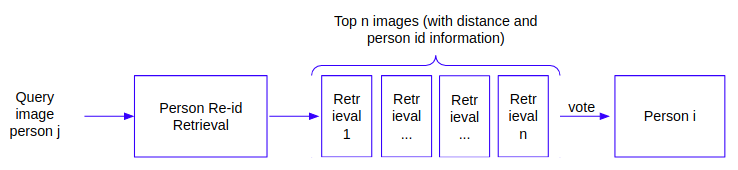
\includegraphics[width=\textwidth]{figures/first_idea.png}

The first problem is how to massage the output of the baseline retrieval system into an output ID $o_i$. Here, we simply take the top $N$ retrievals, and they vote. The winning ID is the one with the most votes. The output of the person ReID system is thus as specified in figure above. Therefore, to learn the observation model, we run the ReID retrieval and voting pipeline on the validation set. The observation model is simply derived from the resulting multi-class $(K-1 \times K)$ confusion matrix. Each cell states how likely an input image of person $j$ is--after the voting procedure--to be classified as class $i$. A trivial application of Bayes' rule gives the posterior over the true class:

\begin{equation}
	\label{eq:first_idea}
	\begin{tabular}{r@{=}l}
		$P(c_j \mid o_i)$ & $\frac{\displaystyle P(o_i \mid c_j) P(c_j)}{\displaystyle\sum_{k=1}^{K} P(o_i \mid c_k) P(c_k)}$ \\ 
	\end{tabular}
\end{equation}

This can easily be extended to a series of query images and the output IDs. Some sequence $x^{1:m}$ of $m$ query images, all of person $j$, is fed to the ReID system. The ReID system produces a corresponding $m$-dimensional vector of classifications $\overrightarrow{o}$. The probability $P(c_j \mid \overrightarrow{o})$ is:

\begin{equation}
	\label{eq:joint_first_idea}
	\begin{tabular}{r@{=}l}
	$P(c_j \mid \overrightarrow{o})$ & $\displaystyle \prod_{k=1}^{m} P(c^k_{j} \mid o^k)$ \\ 
	\end{tabular}
\end{equation}

\noindent with $\overrightarrow{o} = (o^1, \ldots, o^{m})$, and $\overrightarrow{c_j} = (c^1_{j}, \ldots, c^m_{j})$. We could either substitute this into Eq.~\ref{eq:first_idea} or apply it recursively, i.e. applying Bayesian update with each element of the product in turn.%Given this joint probability $P(\overrightarrow{q_j} \mid \overrightarrow{c})$, then we can apply partial observability technique to correct the estimate of who the person might be whenever a series of detections of a person is made.

\section{Vote ratio as observed output}

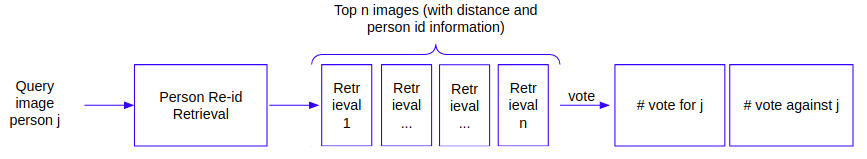
\includegraphics[width=\textwidth]{figures/second_idea.png}

Now, if the person re-id system is specified as in figure above, we can calculate $P(\overrightarrow{v} \mid query = j)$ with $\overrightarrow{v} = <\#vote\_for, ~\#vote\_against>$ by iterating each image of each person on the training set. Using this probability we know how likely that the voting goes right (or wrong) given a query of person $j$. Using this probability we can work out, using Bayesian inference, $P(query=j \mid \overrightarrow{v})$ as:

\begin{equation}
	\label{eq:second_idea}
	\begin{tabular}{r@{=}l}
		$P(query=j \mid \overrightarrow{v})$ & $\frac{\displaystyle P(\overrightarrow{v} \mid query = j) P(query=j)}{\displaystyle\sum_{k=1}^{K} P(\overrightarrow{v} \mid query = k) P(query=k)}$ \\ 
	\end{tabular}
\end{equation}

\noindent with $K$ the total persons.
\\
\\
\noindent \textbf{Problems:}
This idea is a bit odd, it can be seen from equation \ref{eq:second_idea}, because given the configuration voting $<v_f, v_a>$, then we want to know how likely the query person $j$ is. The $P(\overrightarrow{v} \mid query = j)$ seems more like a proportion of voting configuration for each person $j$.

If we just calculate $P(<v_f, v_a>)$, then this just tells us the proportion of the voting configuration based on the training data.

How can we transform this into, perhaps, a ratio of $\displaystyle\frac{P_j}{\Sigma_{i \neq j} P_i}$? 

\section{Vector of distances as observed output}

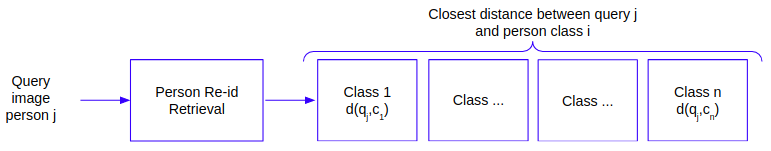
\includegraphics[width=\textwidth]{figures/third_idea.png}

Using the specified re-id system as in figure above with $d(q_j, c_i)$ as the closest distance value between the query of person $j$ and the person classification $c_i$ (the person is classified as $i$), we can calculate the probability $P(d(q_j, c_i) \mid c_i)$ using the (general) distributions over the distance for both matched image and negative images (graphs shown in Figure \ref{fig:match_mismatch_dist}). Using this probability we can work out, using Bayesian inference, $P(c_i \mid d(q_j, c_i))$ as:

\begin{equation}
	\label{eq:third_idea}
	\begin{tabular}{r@{=}l}
		$P(c_i \mid d(q_j, c_i))$ & $\frac{\displaystyle P(d(q_j, c_i) \mid c_i) P(c_i)}{\displaystyle\sum_{k=1}^{n} P(d(q_j, c_k) \mid c_k) P(c_k)}$ \\ 
	\end{tabular}
\end{equation}

\noindent with $n$ the total persons. However, this only works out if the person retrieval system provides the distance $d(q_j, c_i)$ for all $1 \leq i \leq n$ in each query.

\begin{figure*}
	\centering
	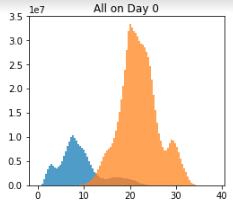
\includegraphics[width=0.40\textwidth]{./figures/match_mismatch_dist.png}
	\caption{Assuming this is a distribution over distance with blue is a distribution for matched query-image ($q_j = c_i$) and orange is a distribution for negative images ($q_j \neq c_i$).}
	\label{fig:match_mismatch_dist}
\end{figure*}

Given particular time interval $m$ where a series of $m$ query images of person $j$ is fed to the system producing distances $d(q_{1j}, c_{1i}), \ldots, d(q_{mj}, c_{mi})$, then the probability $P(\overrightarrow{c_i} \mid \overrightarrow{d(q_j, c_i)})$ can be defined as:

\begin{equation}
	\label{eq:joint_third_idea}
	\begin{tabular}{r@{=}l}
		$P(\overrightarrow{c_i} \mid \overrightarrow{d(q_j, c_i)})$ & $\displaystyle \prod_{k=1}^{m} P(c_{ki} \mid d(q_{kj}, c_{ki}))$ \\ 
	\end{tabular}
\end{equation}

\noindent with $\overrightarrow{c_i} = (c_{1i}, \ldots, c_{mi})$, and $\overrightarrow{d(q_j, c_i)} = (d(q_{1j}, c_{1i}), \ldots, d(q_{mj}, c_{mi}))$.

\end{document}